% 3) Dataset
% - Curlie = community edited web directory -> 3M websites in 92 languages,
% labeled in hierarchical categories, however they only used the top level categories
% Originally, there were 15 top level categories, but they dropped "Regional"
% - Majority of classes associated with Bussiness (27), Society (13.9) or Arts (9)
% - 40% of the websites are in English, 16 % in German, 5% in french, 6% in Japanese
% - Although each page may, in principle, have an arbitrary number of category labels, 
% at the top level, the data is mostly single-labeled, with only 2.1% of samples appearing 
% in two or more taxonomy trees of the 14 top-level classes.


\section{Data}

\textbf{Original data}. In our work, we utilise the crowdsourced annotated Curlie data provided by the authors of Homepage2vec \cite{homepage2vec}. 
This dataset consists of 840 websites, each annotated by three independent annotators instructed to assign one or more of the 14 top-level categories to each website. To assess the level of agreement per website between the annotators, we computed pairwise Cohen's kappa \cite{cohen-coef} accross all three
annotators and aggregated the score via mean. On average, each website has a mean pairwise Cohen's kappa of $0.2 \pm 0.02$ indicating a low level of agreement between the annotators. For each website and category, we assign the given category label if at at least 2 annotators agreed on the label. We decided on this threshold since it resulted in the most realistic number of labels per website ($2.5$), in contrast to agreement of all three labelers ($0.54$) and at least one labeler ($7.66$). For each website, we then scrape the HMTL content and parse it into useful features. We adapt the same feature extraction procedure as in \cite{homepage2vec}. Namely, we extract the top-level-domain, domain, title, description, keywords, first 50 links and first 100 sentences.

% Likely Mika will say we do not need this, and I will likely agree
% I think most imporant information from the table is low number of keywords and descriptions accross all datasets
\begin{table}[!ht]
\centering
\caption{Percentage of websites with each feature accross our datasets.}
\label{tab:feature_information}
\begin{tabular}{lrr}
\toprule
 & Original & Curlie-gpt-10k \\
\midrule
n & 761.00 & 9190.00 \\
tld (\%) & 100.00 & 100.00 \\
domain (\%) & 100.00 & 100.00 \\
tags (\%) & 93.69 & 95.47 \\
titles (\%) & 98.42 & 98.28 \\
descriptions (\%) & 54.93 & 62.95 \\
keywords (\%) & 19.58 & 27.29 \\
links (\%) & 89.88 & 91.62 \\
sentences (\%) & 99.08 & 99.03 \\
\bottomrule
\end{tabular}
\end{table}


\textbf{Additional datasets.} We use the best performing GPT classifier that we asseses against the original dataset with human annotations to label two new datasets. First, \textbf{gpt-data} contains 250 websites that were generated by prompting ChatGPT. This dataset contains generally most popular websites such as \textit{apple.com}, \textit{microsoft.com} etc. Second, \textbf{curlie-gpt-10k} contains randomly selected 10k websites from the Curlie dataset. For both of these datasets, we follow the exact same preprocessing and feature extraction procedure as for the original dataset. Table \ref{tab:feature_information} shows the percentage of websites with each feature accross our datasets. We can see that all websites mostly lack keywords, and descriptions except from the GPT suggested websites. Interestingly, according to homepage2vec \cite{homepage2vec}, keywords yielded the biggest improvement in performance. 

Finally, Figure \ref{fig:class_distribution} shows the class distribution of the original dataset. We can see that the dataset is highly imbalanced with the majority of websites belonging to the \textit{Business} category, followed by \textit{Arts} and \textit{Society}. This issue was pointed in homepage2vec \cite{homepage2vec} and resulted in model's poor performance on minority classes. We will 
address this issue by using class weights during training to penalise model more for misclassifying minority classes.

\begin{figure}[h!]
    \centering
    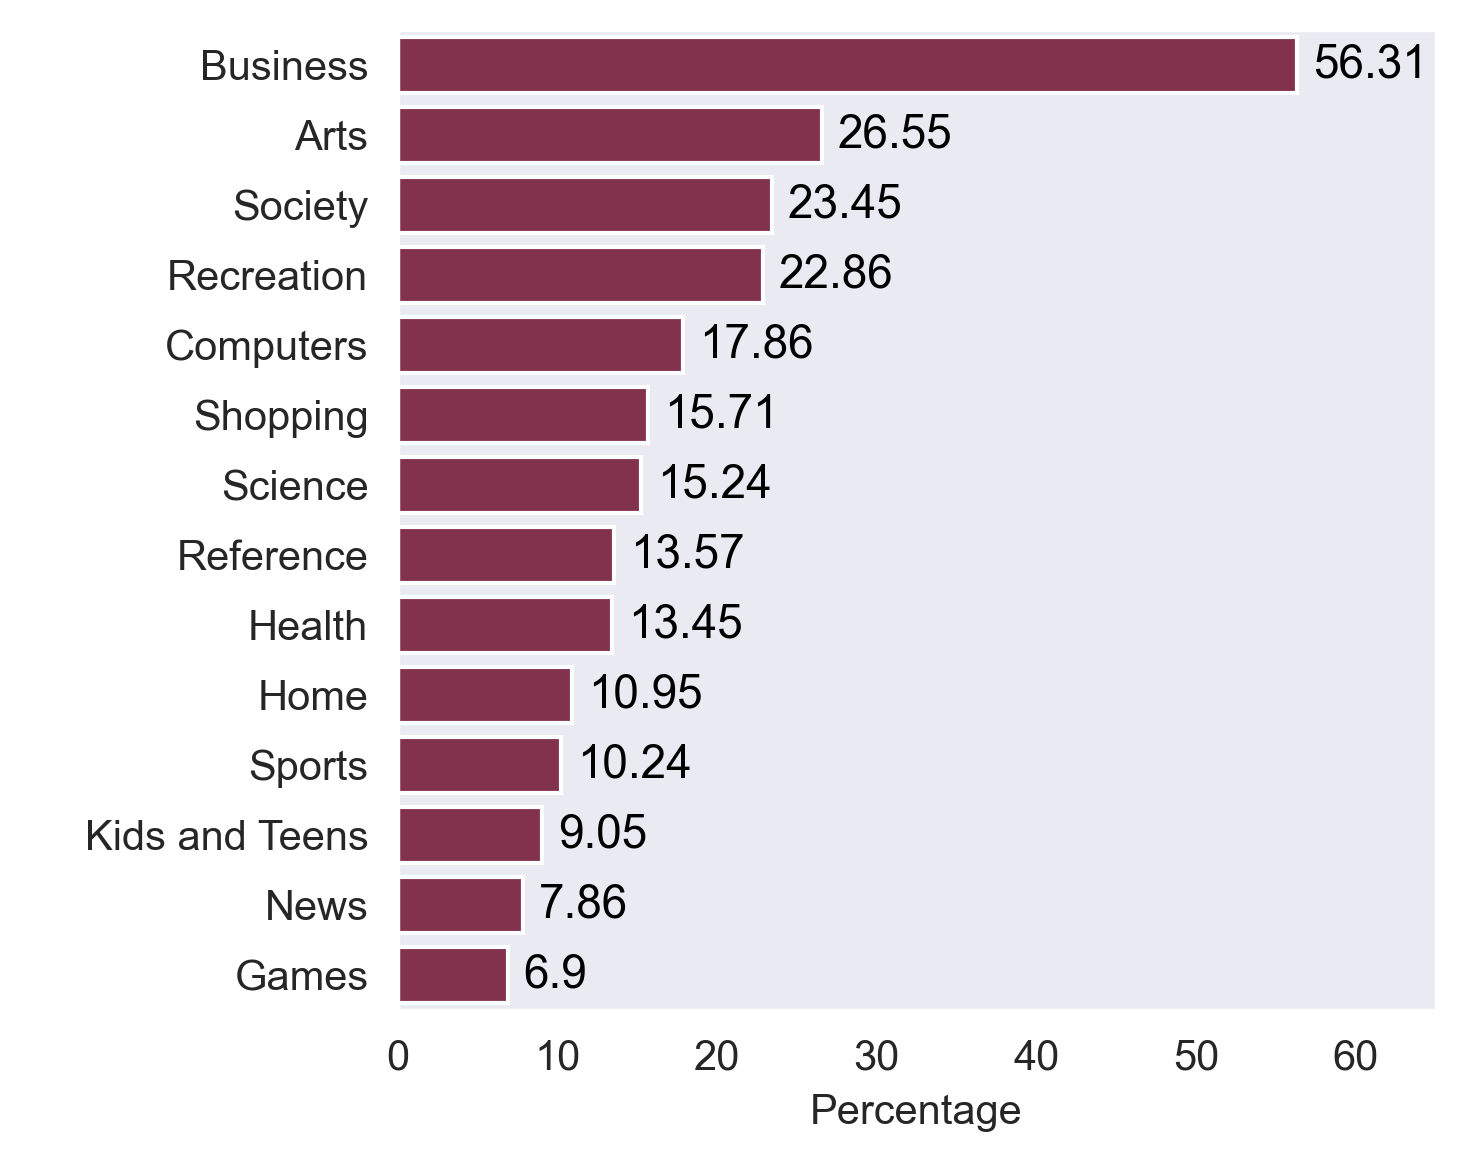
\includegraphics[width=1\columnwidth]{figures/category_distribution.png}
    \caption{Class distribution of the original dataset.}
    \label{fig:class_distribution}
\end{figure}
